% !TeX encoding = UTF-8
% !TeX spellcheck = fr_FR
% !TeX root = ../mythesis.tex
% !TeX program = pdflatex (build)
%%% TeXmaker : no 'magic comments' but set Root with Options > Set as master file

%useful stuff for what follows

\newcommand{\kbf}{\pmb{k}}
\newcommand{\vbf}{\pmb{v}}
\newcommand{\rbf}{\pmb{r}}

\graphicspath{{./}{./fig/}{./chap3_custom_st/fig/}}

\chapter{Optical generation of arbitrary acoustic horizons}

\label{chap:generation_transonic_fluid}

The study of particle creation in the presence of highly curved spacetime has been a subject of interest for many years. The most famous example is the Hawking radiation \cite{hawking_black_1972}, which predicts the creation of particles from the vacuum in the vicinity of a black hole event horizon enabling the black hole 
to evaporate. The obvious difficulty to test this prediction experimentally is double. First, the blackness of such an object makes it hard to spot with a telescope meaning one have to rely rather on the peculiar behavior of visible object moving in the gravitationnal field of such a supermassive object. The optical observation of a black hole took almost one century since the first prediction of gravitationnal collapse by Subrahmanyan Chandrasekhar in 1920. It required 
the synchonization of nine telescope across the world to obtain an optical system whose optical aperture is the size the diameter of earth. the black body temperature of 

As mentionned in the previous chapter, the creation of a sonic horizon in a polariton fluid can lead to spontaneous emission of bogoliubov modes provided the downstream region collective excitation spectrum
exhibits negative energy modes. Furthermore, it was shown that the strength of the emitted signal depends strongly on the curvature of the horizon, or in other words, its steepness. To ensure that particle creation is in principle 
possible to be observed in the lab, one need to fully characterize the mean field of the fluid as well as locally probe its excitation spectrum. This chapter is dedicated to the description of the fully optical generation of arbitrary transonic fluids as well as the characterization of the excitation spectrum on both side of the horizon. 
The latter revealed the first measurement of negative energy modes in a supersonic quantum fluid, validating the possibility to observe particle creation in a polariton fluid.

The first part will focus on the generation of mean fields with arbitrary velocity profile through the shapping of the pump laser phase. In a second part, we will present the pump probe spectroscopy method used to locally measure the collective excitation spectrum as well
as the results obtained on several transonic fluids. The results obtained are reported in Ref ??


\section{Optical generation of arbitrary fluid velocity field}


Let us set the coordinates $x$ and $y$ to describe the microcavity plane. As explained in Chapter 2, translationnal invariance in the $xy$-plane ensure in plane momentum conservation along photonic polaritons excitation while the wavevectors along the
$z$ direction are fixed by the cavity and quantum well length. Furthermore, in this experiment the laser beam is set to be quasi resonant with the lower polariton branch. As a consequence, the transverse phase of the laser is directly imprinted on the polariton field.
Indeed, in the low wavevector limit, the lower polariton branch can be safely approximated by a parabola, namely :

\begin{equation}
    \omega_{LP}(\kbf) = \omega_{LP}^0 + \dfrac{\hbar k^2}{2m_{LP}}.
\end{equation}

The group velocity of a polariton is then $\vbf = \frac{\partial \omega_{LP}}{\partial k} = \frac{\hbar \kbf}{m_{LP}}= \frac{\hbar \kbf_p}{m_{LP}}=$ where $\kp$ is the in plane wavector of the pump laser.
In the case of a plane wave $\kp=\vec{\nabla}\phi(\rbf)$ where $\phi(r)$ is the spatial phase. This can safely be generalized to more complex spatial phase profile.
At the end, we obtain a direct link between the driving laser phase and the velocity of the fluid :

\begin{equation}
    \vbf = \dfrac{\hbar \vec{\nabla} \phi(\rbf)}{m_{LP}} .
\end{equation}

\subsection{Waterfall configuration}


\subsection{Target velocity profile}
Before entering in consideration about whether the fluid cross a critical velocity or not the first task is to be able to generate a fluid with that exhibits two homogeneous regions separated by a sharp transition and yielding two well defined velocities. 
To clarify, let us call the region before the transition the upstream region with velocity $v_{up}$ and the region after the transition the downstream region with velocity $v_d$.
To model this configuration, we arbitrary define a target velocity profile as follow : 

\begin{equation}
    v(x)= \frac{v_{d}-v_{up}}{2}\mathrm{tanh}(\frac{x-x_h}{w_h})+\frac{v_{up}+v_{d}}{2}
    \label{eq:target_velocity}
\end{equation}
where $x_h$ and $w_h$ are the position and width of the transition respectively. This profile is represented in \autoref{fig:target_velocity.pdf} a).
One can then verify that :

\begin{subequations}
    \begin{align}
    &\lim\limits_{x-x_h\ll-w_h} v(x) = v_{up},\\
    &\lim\limits_{x-x_h\gg+w_h} v(x) = v_{d}.
    \end{align}
\end{subequations}

\begin{figure}[h]
    \centering
    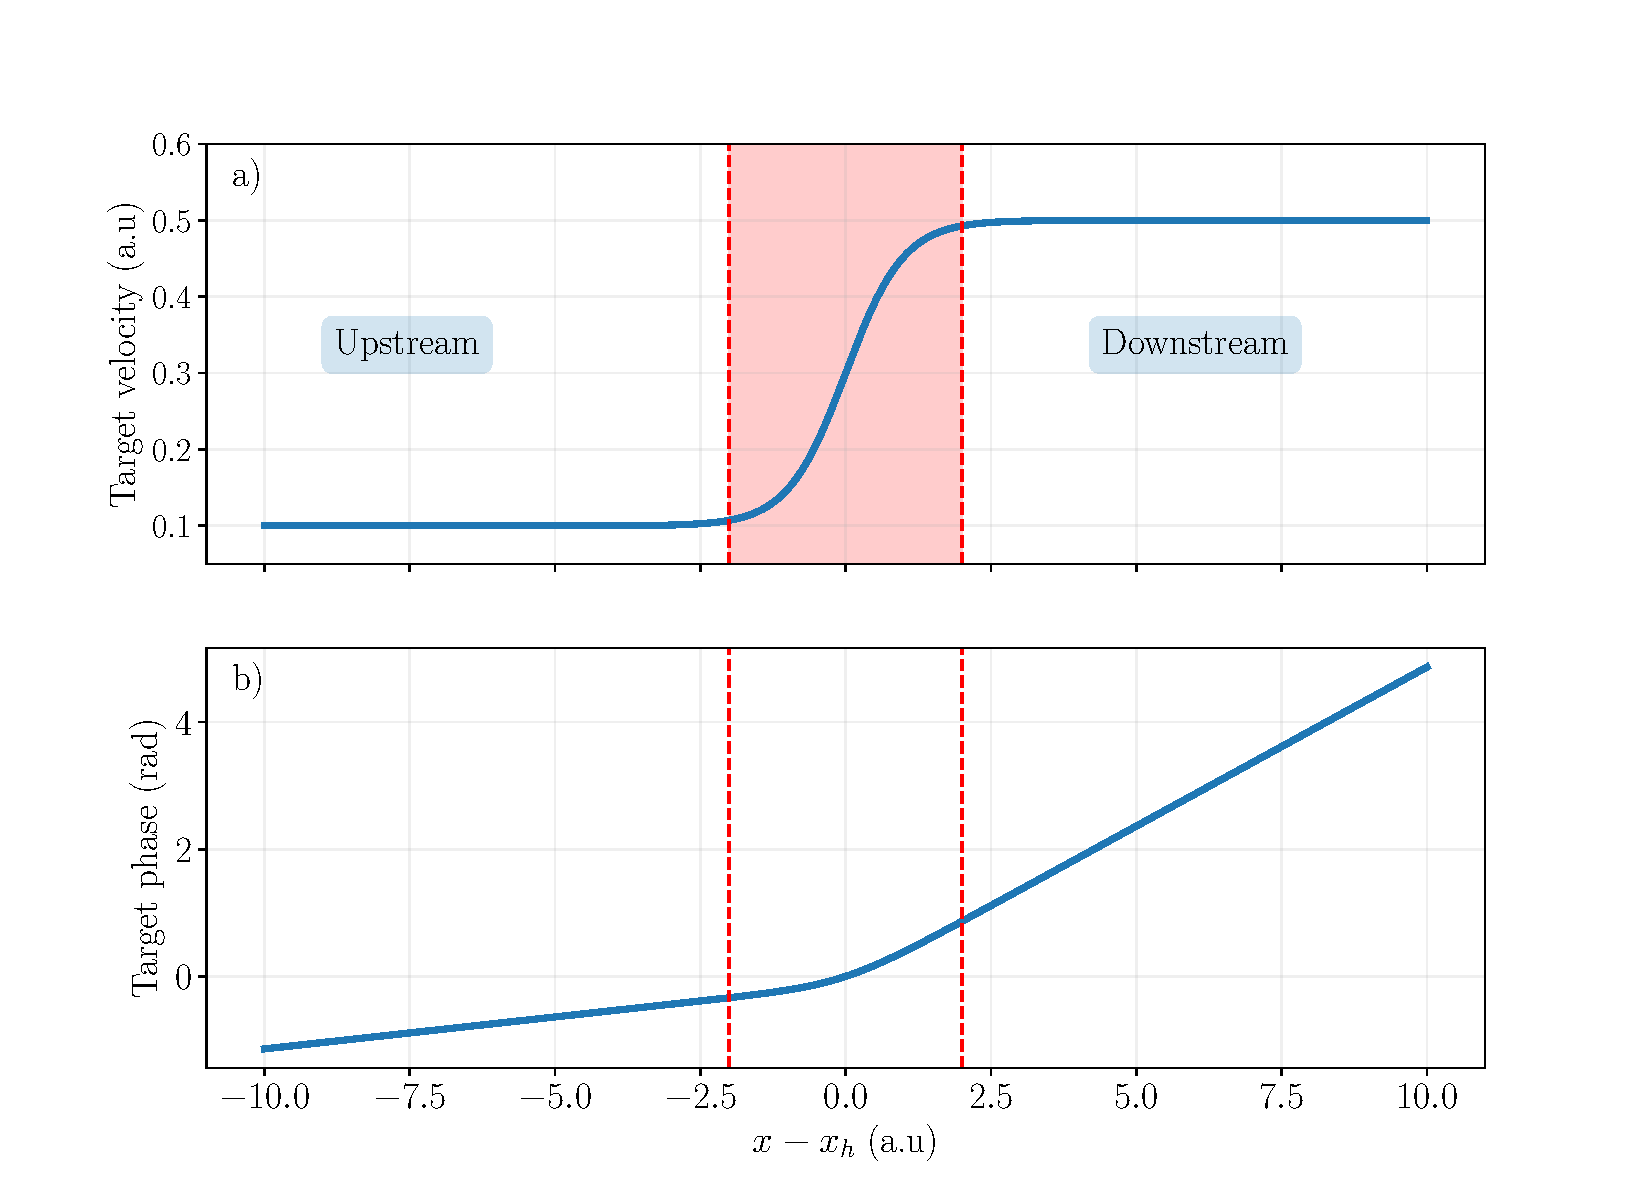
\includegraphics[width=1\textwidth]{chap3_custom_st/fig/target_velocity.pdf}
    \caption{ a) Target velocity profile for input parametes $v_{up}=0.1$, $v_{d}=0.5$, $x_h=0$ and $w_h=1$ in arbitrary units. The red shaded area represent the 
    transition region. b) Corresponding phase profile to be imprinted on the pump laser.}
    \label{fig:target_velocity.pdf}
\end{figure}

Such a velocity profile show a great flexibility in the choice of the upstream and downstream velocities as well as the steepness and the position of the transition. From 
this, one can determine the phase that must be imprinted on the pump laser to generate such a flow profile by simple integration of \autoref{eq:target_velocity}, which gives :

\begin{equation}
    \phi(x) = \dfrac{m_{LP}}{\hbar} \int v(x) dx = \dfrac{m_{LP}}{\hbar} \left( \dfrac{v_{d}-v_{up}}{2} w_h \mathrm{ln}(\cosh(\dfrac{x-x_h}{w_h}))+\dfrac{v_{up}+v_{d}}{2}x \right).
    \label{eq:target_phase_profile}
\end{equation}

The latter is plotted in \autoref{fig:target_velocity.pdf} b). The derivative of this curve at position $x$ gives the the local wavevector of the pump laser or in other words, this curve it represent directly a view side of the wavefront of the driving laser. Indeed, the wavefront is defined as the surface of constant phase of the beam. If we remind that the driving laser has also 
a wavevector along the $z$ direction fixed by the resonant conditions the isophase surfaces are :

\begin{equation}
    \begin{align}
    \phi_{laser}(r)&=k_zz+\phi(x)=cst \\
                      &=\frac{2\pi n_{cav} }{\lambda_0}z+\phi(x)= cst,
    \end{align}
\end{equation}

which is inverted as $z\propto \phi(x)$. To imprint this phase on the pump laser we use a spatial light modulator (SLM) as we will describe in the next section.

\subsection{Wavefront shapping}

Controlling precisely the phase of a laser beam is a common but challenging task in optics. The most basic way to do it is by applying spatial filtering in the fourier plane of a lens.
The phase of the beam is after a second collimating lens is then given by the covolution product of the beam phase and the mask inverse fourier transform. This method then show its limits when one wants to 
generate complex phase profile since its depend on the mask form. A way to overcome this problem is the use of Digital Micromirror Device (DMD) which is an array of micro-mirrors that can be individually controlled to reflect the light or not.
By putting this array in the fourier plan of a lens it is possible to create spatial filtering with arbitrary shapes. However, this method suffers from high losses and diffraction of the light on the individual mirrors that tend to 
add unwanted noise. This being said, DMD are very powerfull devices and allow to do a great amount of things at low cost. A wide range of possible methods are referenced in the great work \cite{wavefront_shapping}. 

\bigskip

\textbf{Spatial light modulator.} In this work, we use a Spatial Light Modulator (SLM) which is a liquid crystal display that can be used to modulate the phase of a laser beam. The principle is to apply a voltage on each pixel of the SLM to change the orientation of the liquid crystal molecules. 
The phase shift is then given by the difference of the optical path of light going through the different pixels as shown in \autoref{fig:SLM}. 

\begin{figure}
    \centering
    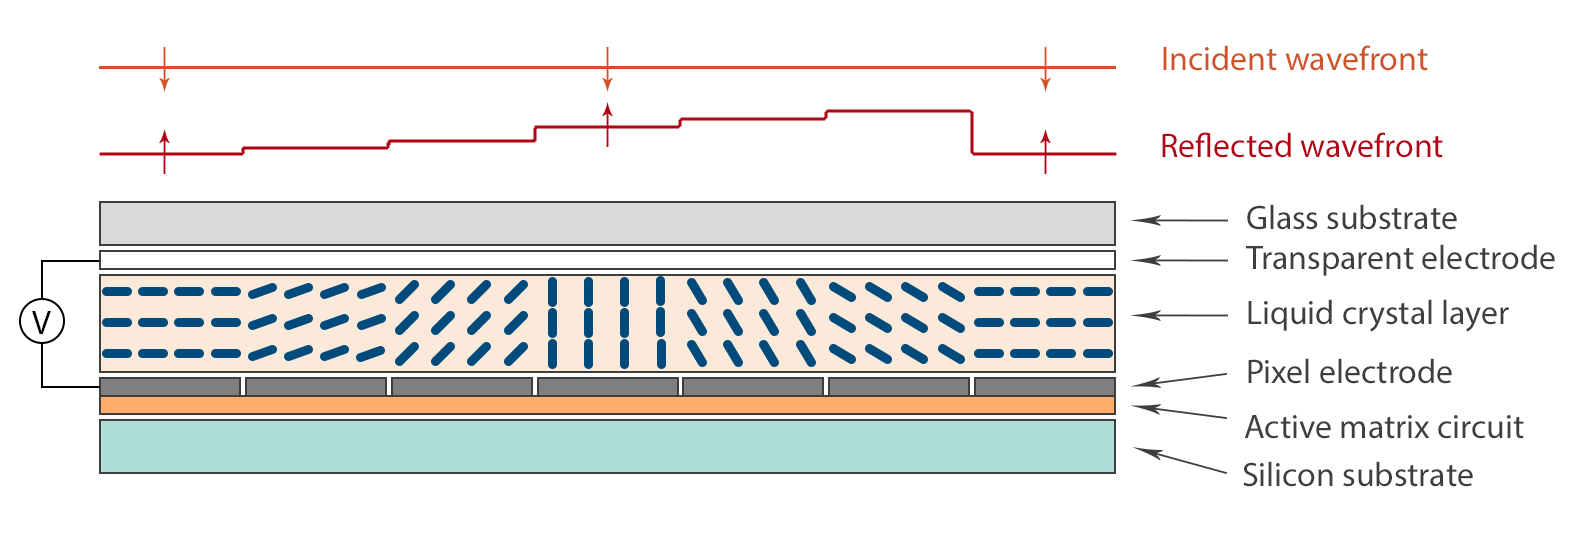
\includegraphics[width=1\textwidth]{chap3_custom_st/fig/SLMprinciple.png}
    \caption{Principle of a Spatial Light Modulator.}
    \label{fig:SLM}
\end{figure}

\noindent By shinning a flat phase collimated beam on the SLM which displays the target phase profile the beam gets reflected carrying the desired wavefront.
However the efficiency of the SLM is not perfect and whenever light is shone on it, some photons migth not see it and not be phase modulated. To overcome this difficulty,
the trick is to first write a blazed phase grating on the SLM screen on top of which the wanted profile is set. All the photons that did interact with the liquid crystals are then mostly diffracted on the first order of the grating. Doing so,
an efficiency of 60-70\% can be reached. This contrast with the usual 80\% usually claimed on manufacturer datasheets that actually correspond to the efficiency in all orders. A typical phase profile imprinted on the SLM is shown
in \autoref{fig:SLM_profile}.



\subsection{Experimental setup}

\begin{figure}
    \centering
    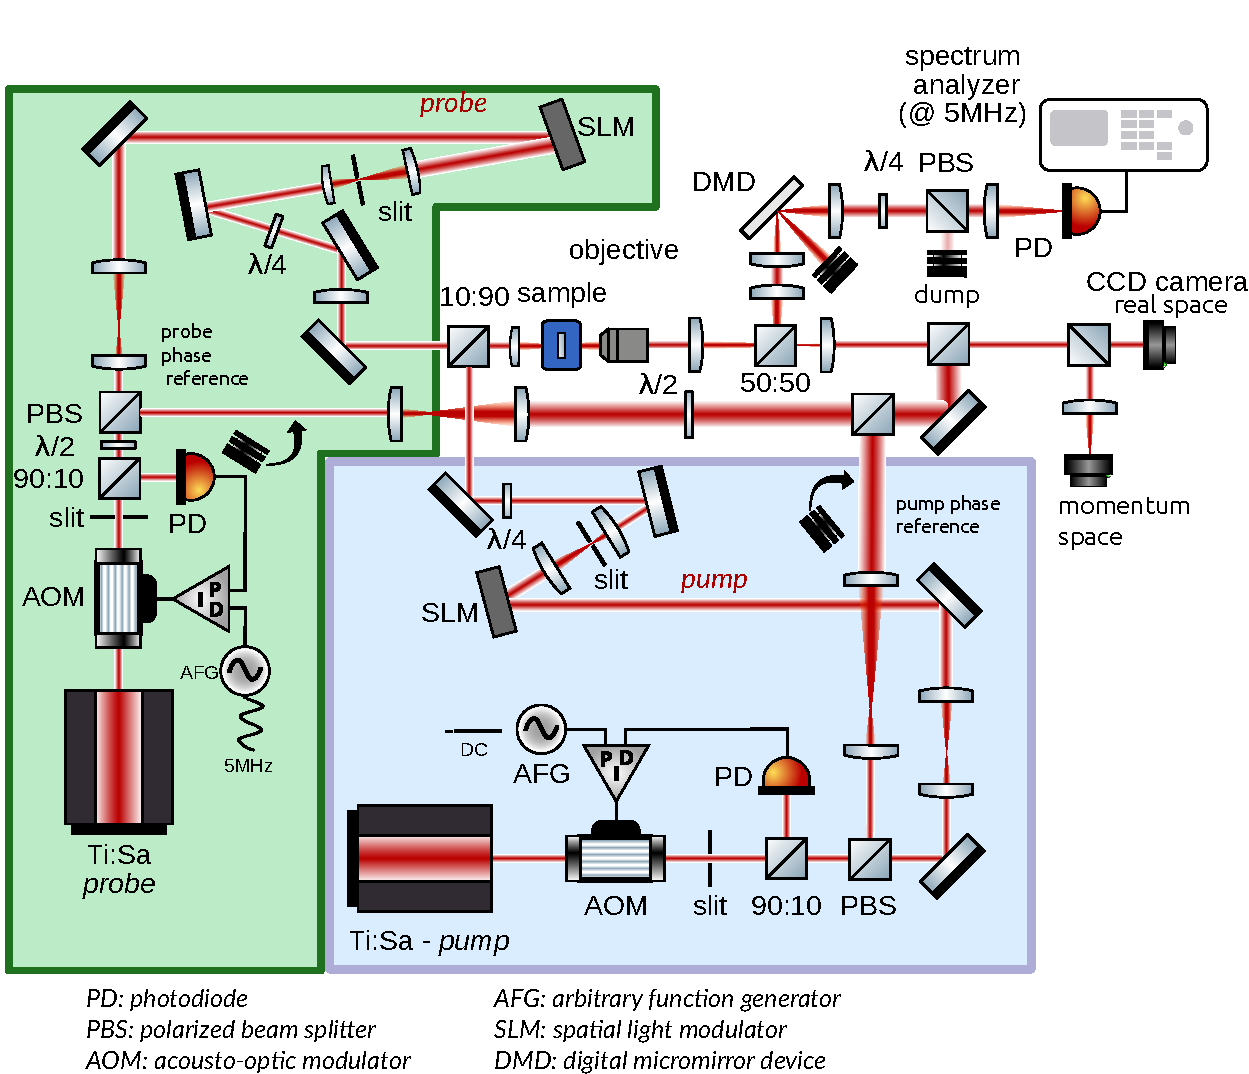
\includegraphics[width=1\textwidth]{chap3_custom_st/fig/set_up_spacetime.pdf}
    \caption{Experimental setup}
    \label{fig:setup}
\end{figure}



